%!TEX root = main.tex
\section{Background and Motivation}
\label{sec:background}


\subsection{The LLM Scheduling Problem}
\label{subsec:problem}

\phm{Demand \emph{uncertainty} and \emph{hybridity} of LLM inference workloads.}
Large language models (LLMs)~\cite{deepseek, llama_official} have nowadays been widely adopted in diverse scenarios like chatbot conversation~\cite{openai_chatgpt}, code generation~\cite{cursor_ai} and embodied intelligence~\cite{wang2023voyager}.
Notably, LLM inferences are conducted in an auto-regressive manner: given a prompt input, each inference task continuously generates new tokens based on its latest token sequence so far---until a special \texttt{<EOS>} token is yielded~\cite{yu2022orca}.
As shown in Fig.~\ref{fig:background_uncertainty}, even a fixed prompt would generate different\footnote{In this paper, we use a temperature of 0.6 in all the inferences, a default setup for many popular LLMs~\cite{llama3_1_8b_instruct,qwen3_32b}.}
output tokens in different runs.
In that sense, the ultimate output length of an inference request can only be known after inference completion, exhibiting strong \emph{uncertainty}.

Apart from demand {uncertainty}, demand \emph{hybridity} is also a distinct property of LLM inference workloads. 
Specifically, during the inference process, each inference commonly caches its token sequence in GPU memory (which is called KVCache~\cite{qin2024mooncake}) to avoid the recomputation overheads; provisioning such a memory space is a prerequisite for inferences to proceed in mainstream LLM frameworks like vLLM~\cite{vllm_v0_8_2}.
%As shown in Fig.~\ref{fig:background_hybridity}, \chen{example describe large KVCache space consumption}
In Fig.~\ref{fig:background_hybridity}, we profile the memory usage and execution time of all the requests respectively from three typical LLM datasets (\emph{as selected} by \cite{hu2024inference})---\emph{SharedGPT}~\cite{sharegpt_vicuna_unfiltered_2025}, \emph{Alpaca-Summarization}~\cite{alpaca_pubmed_summarization_2025}, and \emph{{Document-Write}}~\cite{write_doc_sft_v1_2025}.
It shows both \emph{computation} and \emph{memory} resources are first-class citizens in LLM serving; in contrast, conventional OS workloads are scheduled dominantly based on the computation cost~\cite{cpu_scheduling_comparison_gfg_2026}. %primary computation time are the dominate .
%To summary, resource-demand uncertainty and hybridity are two distinct characteristics of LLM inference workloads.

\begin{figure}[t]
    \centering
    \subfigure[Output length variations of ten randomly sampled prompts from SharedGPT, each collected over 100 inference trial runs.]{
        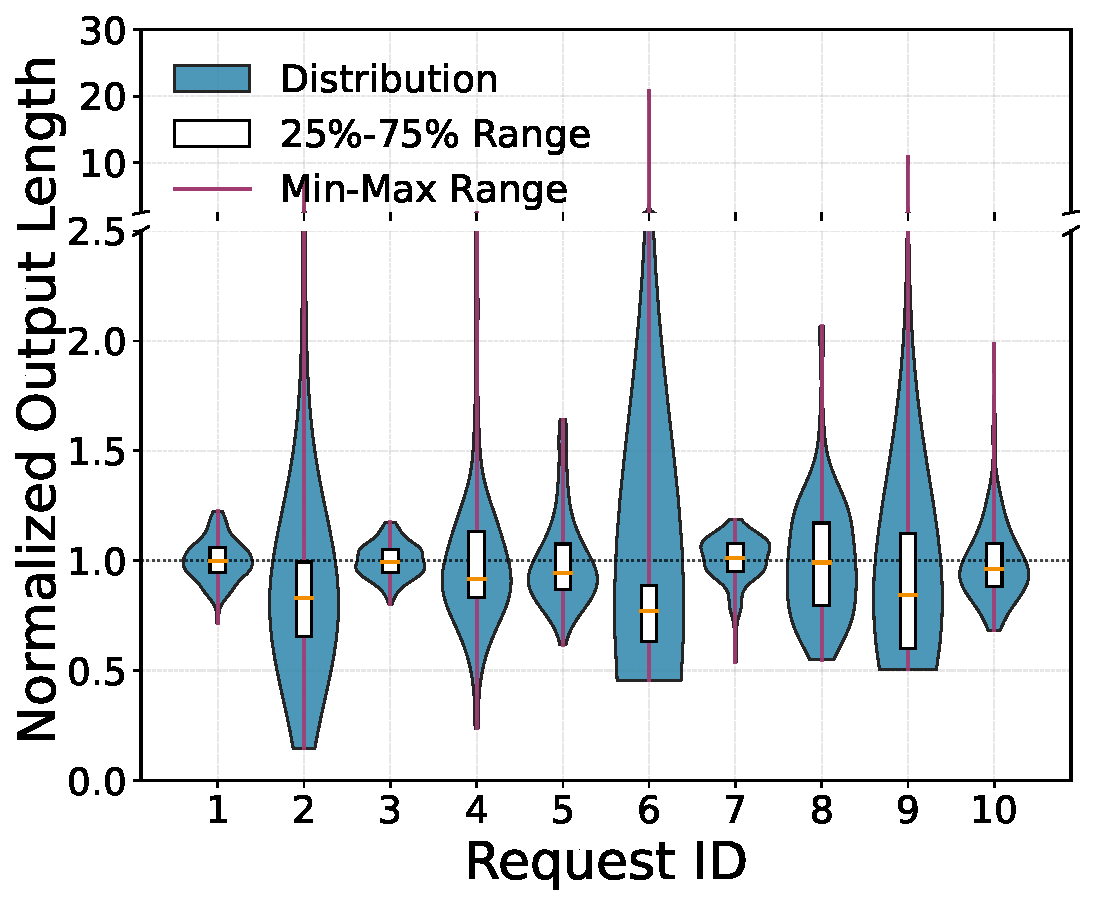
\includegraphics[width=0.45\linewidth]{figures/length_variation.pdf}
        \label{fig:background_uncertainty}
    } %Output length variations of four randomly sampled prompts from SharedGPT, each collected over 100 inference trial runs
    \hfill
    \subfigure[Scatterplot (execution time, peak memory usage) of requests from three datasets, each profiled alone with an H800 GPU.]{
        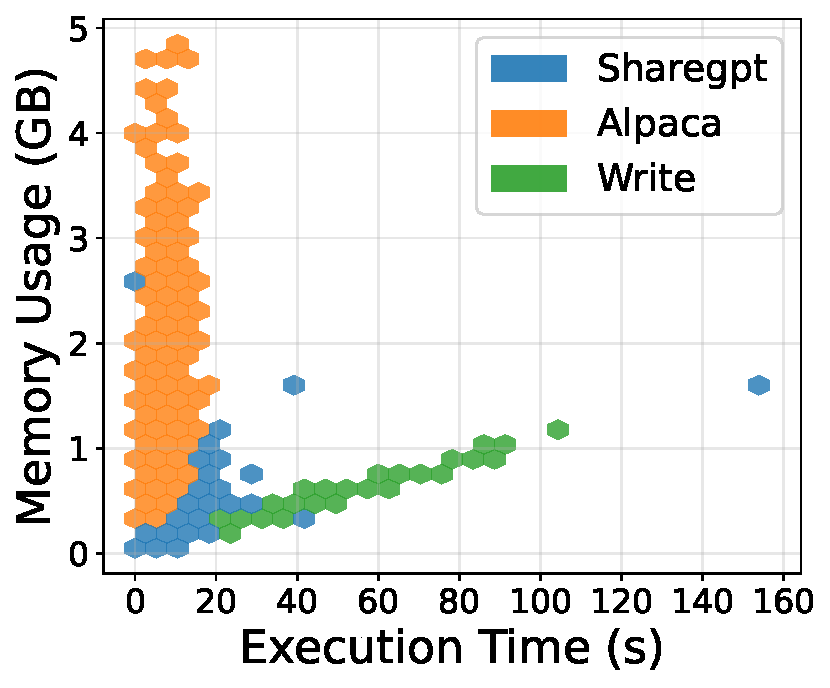
\includegraphics[width=0.45\linewidth]{figures/demand_hybridity.pdf}
        \label{fig:background_hybridity}
    }
    \caption{Empirical evidences on the \emph{uncertainty} and \emph{hybridity} characteristics of LLM inferences' resource demands.}

    \label{fig:background_uncertainty_and_hybridity}
\end{figure}



\phm{Scheduling is crucial on LLM service backends.} 
Given the booming adoption of LLMs, the LLM inference requests from diverse users are often served in a shared backend, where different requests compete for the limited compute and memory resources~\cite{Recasens2025Mind}. 
%\chen{add industrial evidence from mooncake}. 
%{These become the primary bottlenecks for LLM inference as described in the IBM's research~\cite{Recasens2025Mind}.}
For good user experience, it is crucial to properly schedule the LLM inferences to achieve low overall latency. 
Specifically, while there are diverse latency metrics for LLM inferences: time-to-first-token (TTFT), time-per-output-token (TPOT), and time-to-last-token (TTLT), in this paper we primarily focus on TTLT due to its comprehensiveness\footnote{
First, TTLT is increasingly significant for many scenarios like agentic AI: for example, for  LLM-powered robotic control~\cite{chen2023typefly,wang2024llm}, downstream operations can only be launched after LLM generation completion. % yielding the entire output sequence.
Second, optimizing TTLT often also helps to reduce the other metrics.
For TTFT, by avoiding head-of-line-blocking, TTLT-friendly schedulers can naturally improve TTFT (as confirmed by our later evaluation);
for TPOT---which in statistical analysis is often defined as \emph{dividing TTLT by the output token length}~\cite{wu2023fast,fu2024efficient}---reducing TTLT would proportionally improve TPOT.
}, as in a series of existing works~\cite{shahout2024don,qiu2024efficient}. %,fu2024efficient}.~\chen{add citations wherever appropriate}



\subsection{Limitations of Existing LLM Schedulers}
\label{subsec:limitations}

In the literature, a series of schedulers have been proposed for LLM inference workloads.
Confronting demand uncertainty, early-stage LLM schedulers usually employ \emph{demand-agnostic} scheduling heuristics. 
Production LLM frameworks like vLLM~\cite{kwon2023efficient} and SGLang~\cite{zheng2024sglang} employ a simple \emph{first-come-first-serve} (FCFS) scheduler, which suffers the head-of-line-blocking problem.
To address that problem, FastServe~\cite{wu2023fast} adopts a \emph{multi-level feedback queue} (MLFQ) to periodically degrade ongoing inferences to lower priorities after fixed service quantums---essentially approximating (yet not as good as) \emph{shortest-remaining-processing-time} (SRPT) at the cost of additional preemption overheads.

Noticing the deficiencies of \emph{demand-agnostic} schedulers, recent LLM schedulers adopt a \emph{prediction-based} methodology.
For example, the \emph{Speculative Shortest Job First} (SSJF)~\cite{qiu2024efficient} scheduler approximates \emph{shortest-job-first} (SJF) by using a fine-tuned BERT-base model, which predicts the output token length given the inference prompt.
In the meantime, Fu~\emph{et~al.}~\cite{fu2024efficient} also approximate SJF using an OPT-125M model, which predicts the requests' relative output-length \emph{rank} (rather than the exact lengths).
Recently, the TRAIL work~\cite{shahout2024don} approximates SPRT with an MLP model, which predicts the output length continuously at iteration granularity---using the feature embeddings of certain LLM layers.  

\begin{figure}[t]
    \centering
    \subfigure[Predicting a single (bucket) value fails to cover all output-length possibilities; each bucket represents an output-length range of {100} tokens.]{ %capture Accuracy Degradation under Output Uncertainty]{
        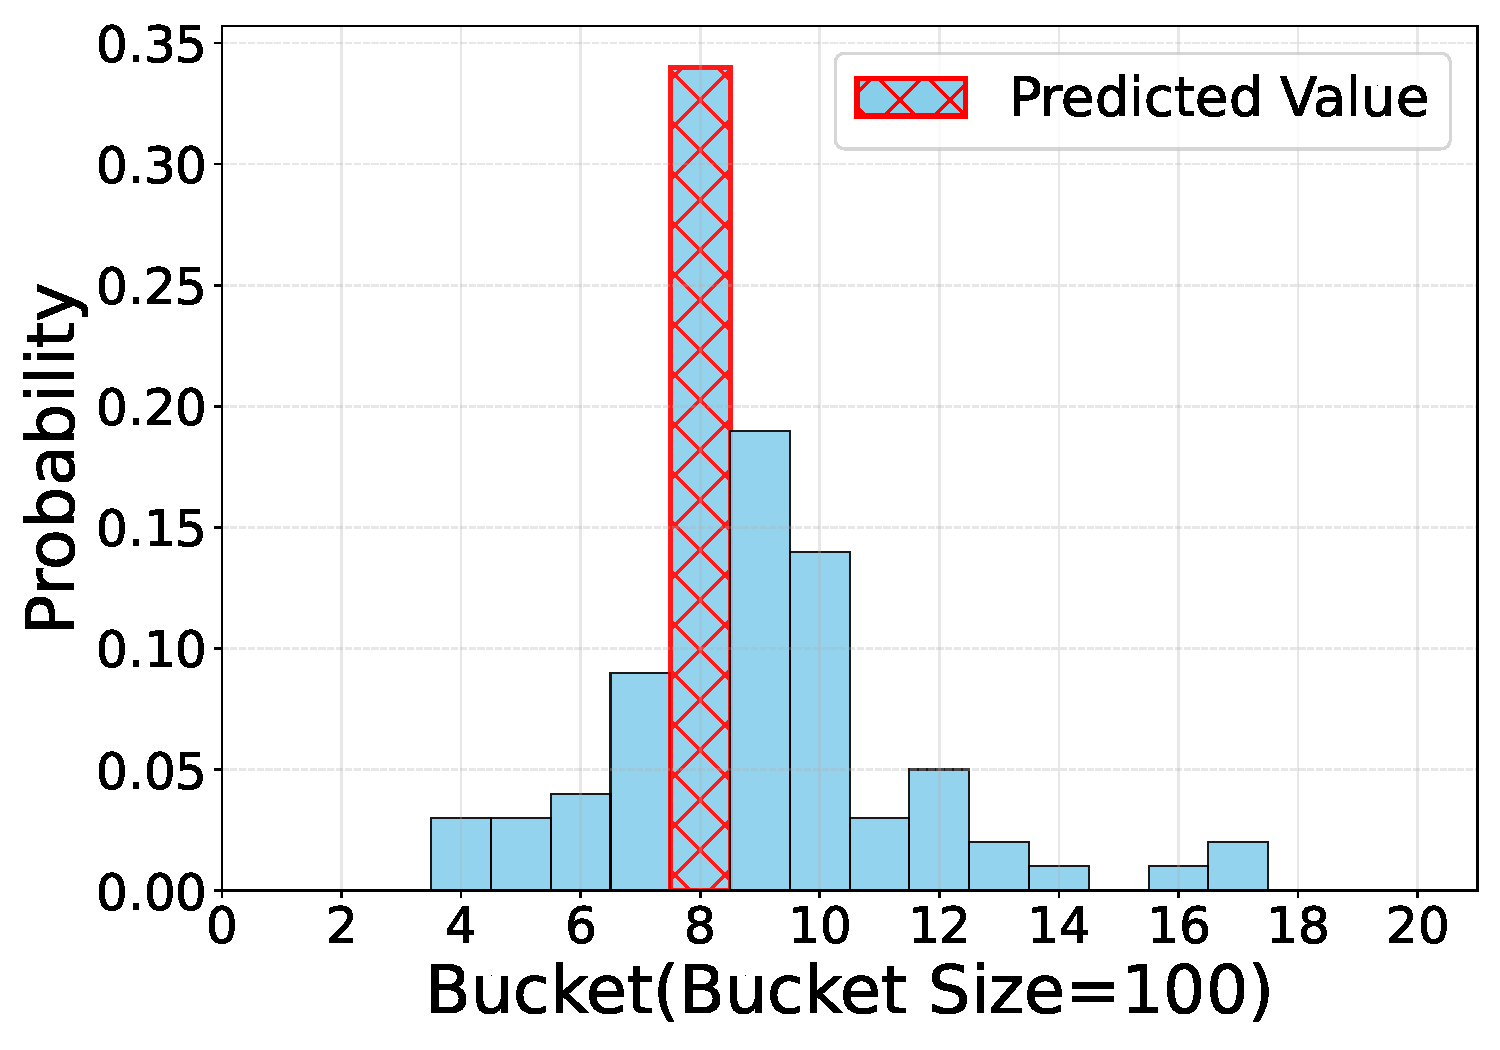
\includegraphics[width=0.53\linewidth]{figures/motivation_low_accuracy.pdf}
        \label{fig:low_prediction_accuracy}
    }
    \hfill
    \subfigure[Due to KVCache constraints, prioritizing requests with shorter outputs may be suboptimal.]{ % Suboptimality of SJF Based on Execution Time]{
        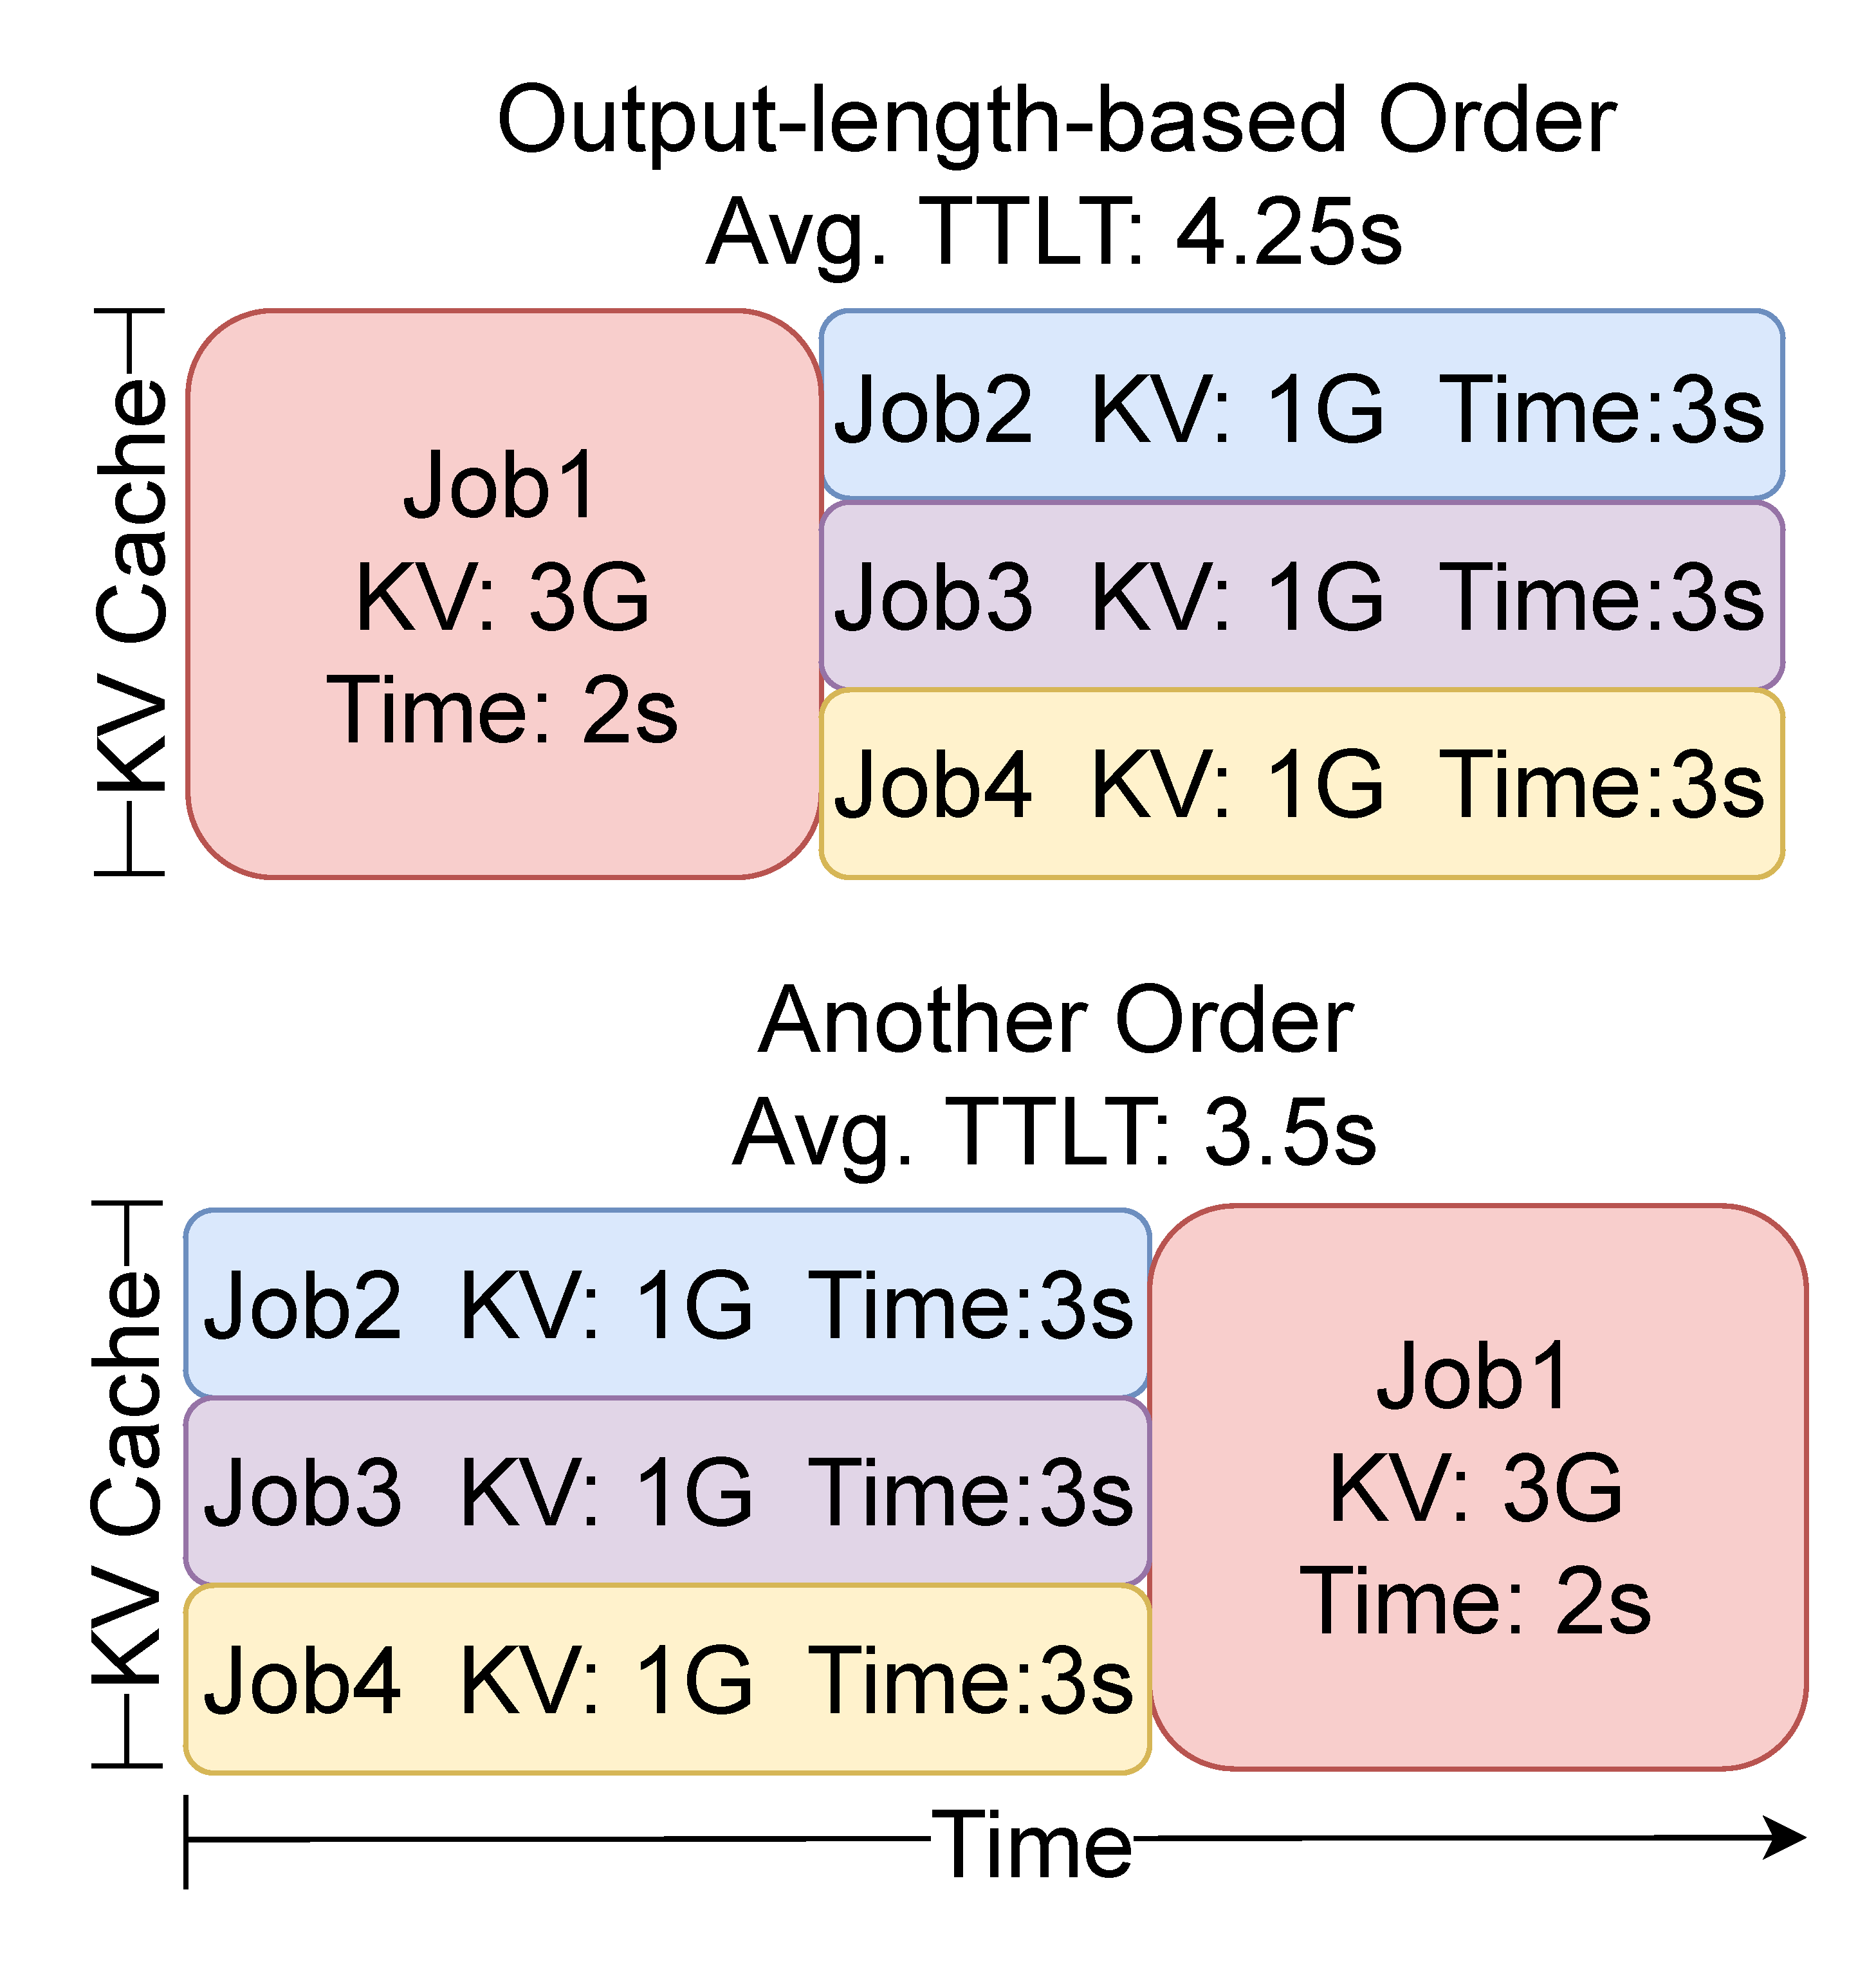
\includegraphics[width=0.37\linewidth]{figures/suboptimality_SJF.pdf}
        \label{fig:wrong_scheduling_order}
    }
    \caption{Examples elaborating the deficiencies of existing schedulers when confronting demand uncertainty and hybridity.} 
    \label{fig:deficiencies}
\end{figure}


However, the above prediction-based schedulers still fall short in handling demand \emph{uncertainty}.
First, their length predictors commonly require heavy-weight offline training (fine-tuning typically requires collecting and processing 10k+ training examples~\cite{jin2023s, fu2024efficient}), and the model trained for one LLM cannot be directly applied for another.
Second, those output-length predictors yield a \emph{single} prediction value, losing valuable probabilistic distribution information.
In fact, demand uncertainty is a built-in property of LLM inferences, and a single prediction value would hardly be accurate in reality. 
As shown in Fig.~\ref{fig:low_prediction_accuracy}, 
%given the ground-truth on output-length distribution (obtained by repeating the same prompt for 100 times), 
the single value predicted by DistillBert as in \cite{qiu2024efficient} only achieves an accuracy of 34.1\% (by hitting only one out of the totally {20} buckets).
As we show later in Sec.~\ref{subsec:gittins}, preserving the length distribution can help to make better scheduling decisions. 
Therefore, in handling demand uncertainty, we need to design a \emph{training-free} method that directly predicts the output-length \emph{distribution}.

Meanwhile, we note that those schedulers also fall short in handling demand \emph{hybridity}. 
They quantify an LLM request's service cost merely as its computation time (represented by its output token length), being inaccurate by neglecting its resource consumption of GPU memory. 
In fact, since both the input and output tokens take up KVCache spaces during inference, two inferences with the same output length may exhibit substantially different memory costs.  
As shown in Fig.~\ref{fig:wrong_scheduling_order},  when the service backend is bottlenecked on GPU memory, simply prioritizing the LLM inferences with shorter output lengths may in fact be suboptimal. % in terms of the average TTLT performance. 
Therefore, to handle demand hybridity of LLM inferences, we need to jointly consider their resource consumptions in both compute and memory dimensions.

To summarize, due to demand uncertainty and hybridity, existing LLM schedulers fail to achieve high overall efficiency. 
We next devise a novel scheduler for efficient LLM scheduling, with optimizations respectively in output-length prediction, cost modeling and request queuing. 